% !TEX TS-program = pdflatex
% !TEX encoding = UTF-8 Unicode


\documentclass{beamer}


\mode<presentation>
{
  \usetheme{Warsaw}
  \useoutertheme{infolines}

  \setbeamercovered{transparent}
}


\usepackage[english]{babel}

\usepackage[utf8]{inputenc}

\usepackage{times}
\usepackage[T1]{fontenc}




\title[Characterizing Features of Silicon Wafers] % (optional, use only with long paper titles)
{Characterizing Features of Silicon Wafers}
\date{September 27, 2016}

\subtitle
{using Fourier Transforms and Delaunay Triangulation } % (optional)

\author[Adam Dicken] % (optional, use only with lots of authors)
{Adam~Dicken}
% - Use the \inst{?} command only if the authors have different
%   affiliation.


\subject{Talks}
% This is only inserted into the PDF information catalog. Can be left
% out. 



% If you have a file called "university-logo-filename.xxx", where xxx
% is a graphic format that can be processed by latex or pdflatex,
% resp., then you can add a logo as follows:

% \pgfdeclareimage[height=0.5cm]{university-logo}{university-logo-filename}
% \logo{\pgfuseimage{university-logo}}



% Delete this, if you do not want the table of contents to pop up at
% the beginning of each subsection:
\AtBeginSection[]
{
	\frame{\tableofcontents[currentsection]} 
}


% If you wish to uncover everything in a step-wise fashion, uncomment
% the following command: 

%\beamerdefaultoverlayspecification{<+->}


\begin{document}

\begin{frame}
  \titlepage
\end{frame}

  
  % You might wish to add the option [pausesections]



% Since this a solution template for a generic talk, very little can
% be said about how it should be structured. However, the talk length
% of between 15min and 45min and the theme suggest that you stick to
% the following rules:  

% - Exactly two or three sections (other than the summary).
% - At *most* three subsections per section.
% - Talk about 30s to 2min per frame. So there should be between about
%   15 and 30 frames, all told.

\section{Background}

\subsection{AZ Electronic Materials}

\begin{frame}{AZ Electronic Materials}
	\begin{itemize}
		\item
		Manufacturer of materials for chip makers (processors etc.)
		\item
		Also do R\&D in new methods of chip design
		\item 
		Internship with R\&D team to build a method for reliably characterizing research samples
	\end{itemize}
\end{frame}

\subsection{Self Assembly}

\begin{frame}{Self Assembly}

 \begin{itemize}
  \item
    Traditionally wafers are patterned using lithography
  \item
    Self assembly is a different approach 
  \item
   Two immiscible monomers polymerize to create a \textbf{Block Co Polymer (BCP)} with two distinct ends
   % Can think of this like oil and water
   \item
    Given opportunity system assembles to \textbf{minimize energy}

  \end{itemize}

\begin{center}
  \begin{tabular}{ccc}
  	     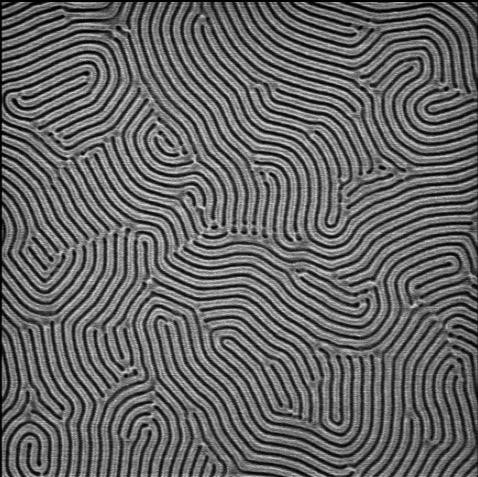
\includegraphics[height=80pt]{images/FFT_in.jpeg}  & 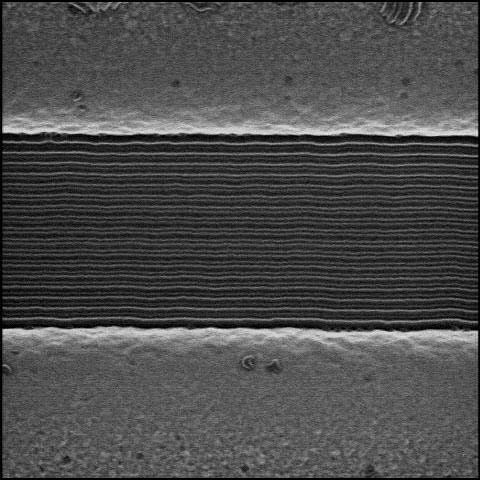
\includegraphics[height=80pt]{images/image16.jpeg} & 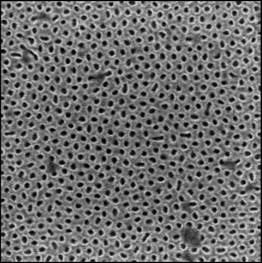
\includegraphics[height=80pt]{images/image10.jpeg}
  \end{tabular}
\end{center}

\end{frame}


\subsection{Data Set}

\begin{frame}{Data Set}

\begin{itemize}
	\item
	Images of wafers from an Electron Microscope
	\item
	Typically 480 x 480 pixels with known field of view (nm)
	\item
	Can think of as just a matrix of intensity values (0-255)
\end{itemize}

\begin{center}
	\begin{columns}
		\column{.5\textwidth}
		\begin{figure}
			\includegraphics[height=80pt]{images/ch.jpg}  
		\end{figure}

		\column{.5\textwidth}
				\begin{table}[]
					\centering
					\resizebox{\textwidth}{!}{%
						\begin{tabular}{llllllllll}
							82  & 73  & 93  & 90  & 86  & 102 & 105 & 115 & 120 & 134 \\
							104 & 109 & 124 & 106 & 92  & 96  & 101 & 129 & 106 & 100 \\
							78  & 99  & 106 & 76  & 65  & 69  & 82  & 137 & 131 & 110 \\
							105 & 118 & 97  & 42  & 26  & 22  & 28  & 91  & 112 & 103 \\
							138 & 134 & 93  & 29  & 13  & 8   & 8   & 63  & 100 & 119 \\
							114 & 105 & 76  & 22  & 3   & 1   & 2   & 45  & 97  & 131 \\
							107 & 107 & 108 & 63  & 21  & 7   & 6   & 36  & 138 & 159 \\
							102 & 120 & 156 & 131 & 80  & 66  & 74  & 102 & 129 & 132 \\
							124 & 117 & 143 & 138 & 152 & 168 & 194 & 165 & 137 & 102 \\
							132 & 121 & 144 & 130 & 124 & 122 & 147 & 128 & 101 & 66 
						\end{tabular}%
					}
				\end{table}
	\end{columns}
\end{center}


\end{frame}


\section{Analysis - Lines}

\subsection{Fingerprint vs DSA}

\begin{frame}{Characterizing}
	\begin{itemize}
		\item
		Characterized by the distance between the lines 
		\begin{math}
			L_{0}
		\end{math}
		\item
		Easy to think of a method to measure Directed Assembly
		\begin{center}
			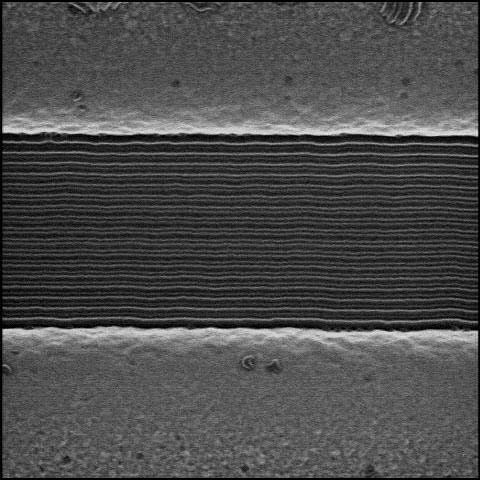
\includegraphics[height=80pt]{images/image16.jpeg}
		\end{center}		
		\item
		Unguided assembly (finger print pattern) is more tricky
		\begin{center}
				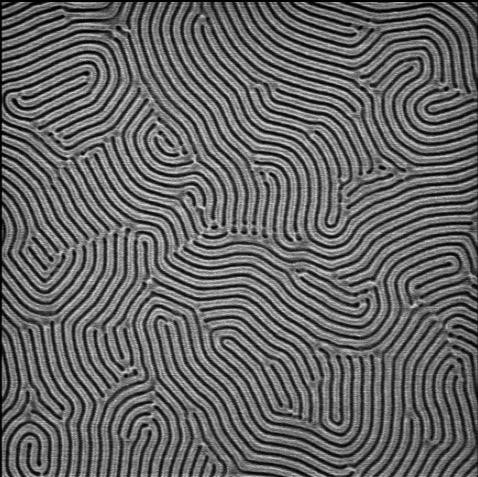
\includegraphics[height=80pt]{images/FFT_in.jpeg}
		\end{center}
	\end{itemize}
\end{frame}


\subsection{Fourier Transform - Motivation}

\begin{frame}{Fourier Theorem}
	\begin{quotation}
	Any well behaved function can be expressed as a combination of sine and cosine waves.		
	\end{quotation}
	\begin{itemize}
		\item
		Pixel data is discretized
		\item 
		We will use a 2D DFFT
	\end{itemize}
\end{frame}

\begin{frame}{Fourier Transform}{Example}
\begin{figure}
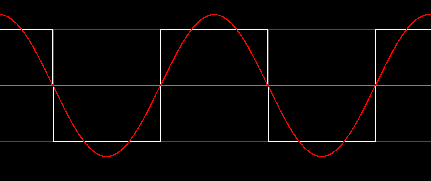
\includegraphics[scale=0.75]{images/image19.png}
\caption{N=1}
\end{figure}
\end{frame}

\begin{frame}{Fourier Transform}{Example}
\begin{figure}
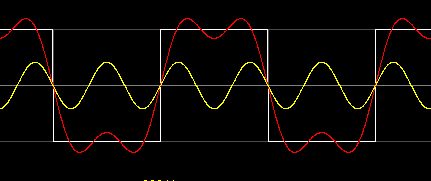
\includegraphics[scale=0.75]{images/image20.png}
\caption{N=2}
\end{figure}
\end{frame}

\begin{frame}{Fourier Transform}{Example}
\begin{figure}
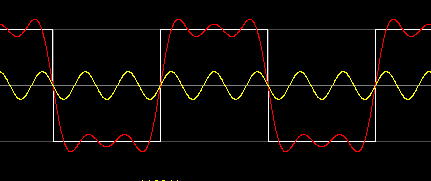
\includegraphics[scale=0.75]{images/image21.png}
\caption{N=3}
\end{figure}
\end{frame}

\begin{frame}{Fourier Transform}{Example}
\begin{figure}
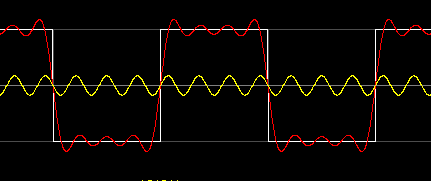
\includegraphics[scale=0.75]{images/image22.png}
\caption{N=4}
\end{figure}
\end{frame}

\begin{frame}{Fourier Transform}{Example}
\begin{figure}
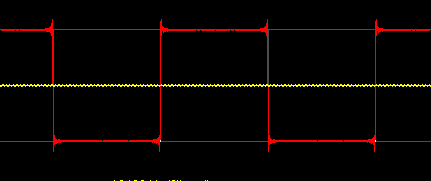
\includegraphics[scale=0.75]{images/image23.png}
\caption{N=Lots!}
\end{figure}
\end{frame}

\subsection{Fourier Transform -  Output}
\begin{frame}{Power Spectrum - 2D}
\begin{columns}
	\column{.5\textwidth}
		\begin{itemize}
			\item
			Output is a map of amplitudes
			\item
			Frequencies which best fit the image in x and y axis
			\item
			Circular spectrum confirms the same frequency in all directions
			\item
			\begin{math}
				f = \sqrt{f_{x}^2 + f_{y}^2}
			\end{math}
		\end{itemize} 
	\column{.5\textwidth}
		\begin{figure}
			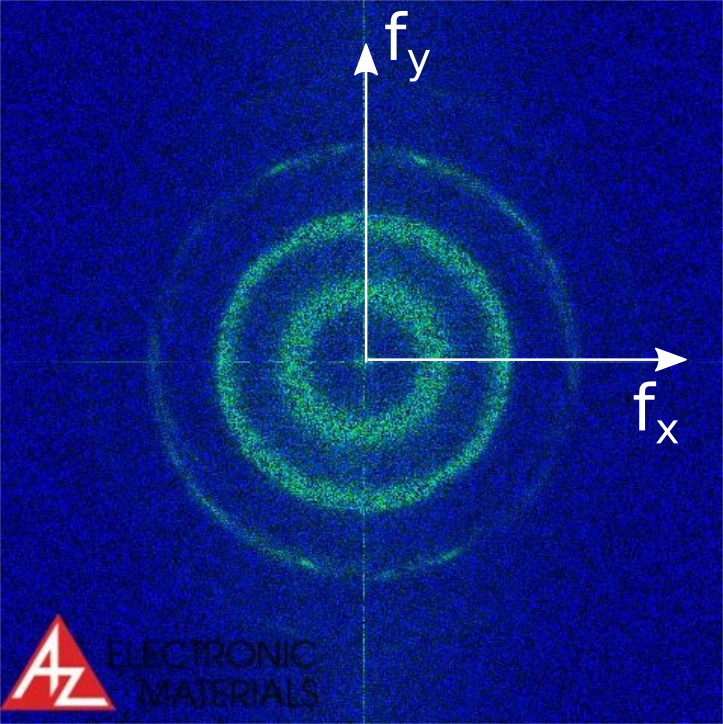
\includegraphics[height=150pt]{images/Fourier-output-axes.png}
		\end{figure}
\end{columns}

\end{frame}

\begin{frame}{Frequency Distribution}
	
	\begin{columns}
		\column{.3\textwidth}
			\begin{figure}
				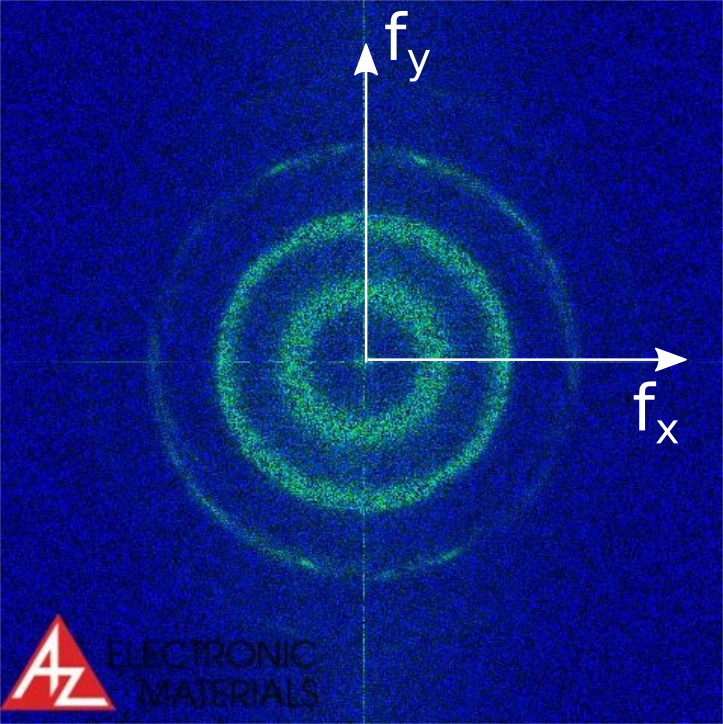
\includegraphics[height=70pt]{images/Fourier-output-axes.png}
			\end{figure}
		\column{.7\textwidth}
			\begin{figure}
				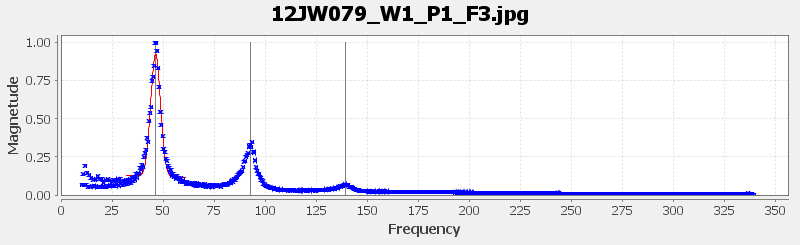
\includegraphics[height=65pt]{images/image34.png}
			\end{figure}
	\end{columns}

	\begin{columns}
		\column{.5\textwidth}
		\begin{itemize}
			\item
			Multiple peaks - harmonics
			\item
			Gaussian fit gives the peak frequency and associated error
			\begin{math}
				f_{0}
			\end{math}
		\end{itemize}
		\column{.5\textwidth}
			\begin{figure}
				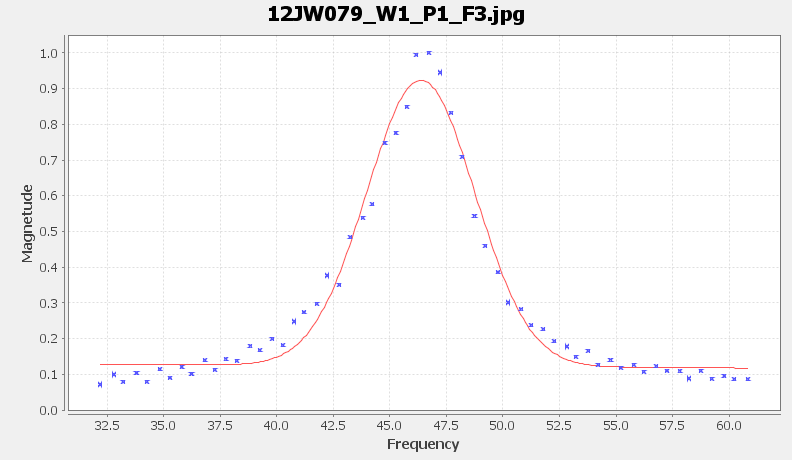
\includegraphics[height=80pt]{images/gaussian_fit.png}
			\end{figure}
	\end{columns}
			
\end{frame}

\begin{frame}{Calculating $L_{0}$}
	\begin{columns}
		\column{.5\textwidth}
		\begin{itemize}
			\item
			Measure peak frequency for multiple images
			\item
			Calculate the mean ($\bar{f_{0}}$) and combine errors
			\begin{displaymath}
			 	\Delta f_{0} = \frac{\sqrt{\sum\limits_{i=1}^N  \Delta f_{0_{i}} }}{N}
			\end{displaymath}
			\begin{displaymath}
				\bar{L_{0}} = \frac{FOV}{\bar{f_{0}}}
			\end{displaymath}
			
		\end{itemize}
		\column{.6\textwidth}
			\begin{figure}
				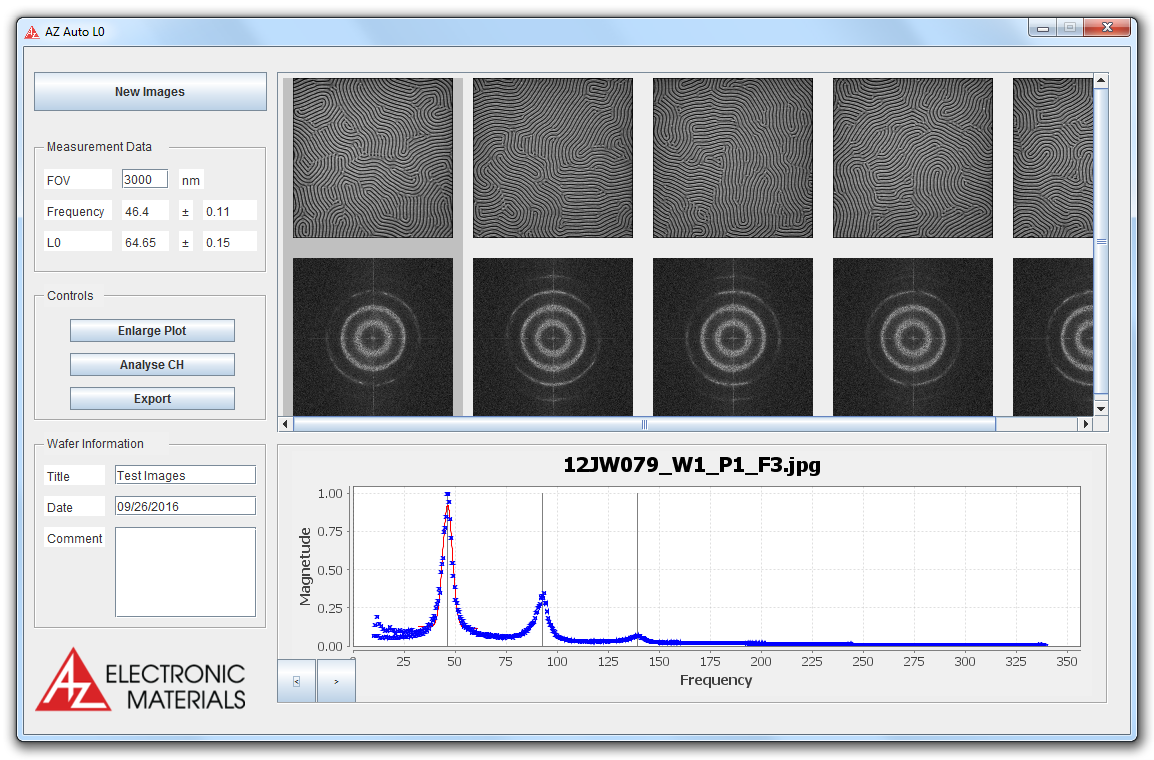
\includegraphics[height=120pt]{images/measuring_l0.png}
			\end{figure}
			
	\end{columns}

\end{frame}

\section{Analysis - Holes}

\subsection{Finding Holes}

\begin{frame}{Finding Holes}
\begin{columns}
	\column{.6\textwidth}
	\begin{itemize}
		\item
		First need to define holes in the image
		\item 
		Simple idea - focus on darkest pixels and expand out to find a hole
		\item
		Stop when next change to next pixel is above a specific threshold
	\end{itemize}
	\column{.4\textwidth}
		\begin{figure}
			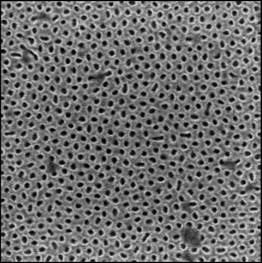
\includegraphics[height=120pt]{images/image10.jpeg}
		\end{figure}
\end{columns}

\end{frame}

\begin{frame}{Finding Holes - Example}
	\begin{figure}
		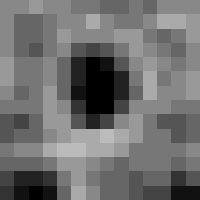
\includegraphics[height=150pt]{images/image38.jpg}
	\end{figure}
\end{frame}
\begin{frame}{Finding Holes - Example}
	\begin{figure}
		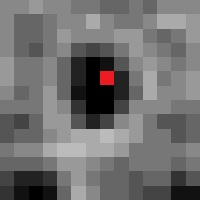
\includegraphics[height=150pt]{images/image39.jpg}
	\end{figure}
\end{frame}
\begin{frame}{Finding Holes - Example}
	\begin{figure}
		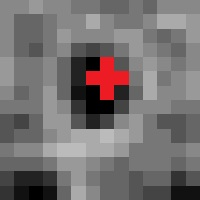
\includegraphics[height=150pt]{images/image40.jpg}
	\end{figure}
\end{frame}
\begin{frame}{Finding Holes - Example}
	\begin{figure}
		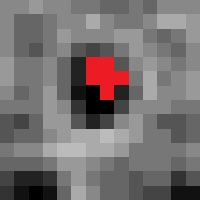
\includegraphics[height=150pt]{images/image41.jpg}
	\end{figure}
\end{frame}
\begin{frame}{Finding Holes - Example}
	\begin{figure}
		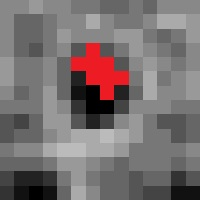
\includegraphics[height=150pt]{images/image42.jpg}
	\end{figure}
\end{frame}
\begin{frame}{Finding Holes - Example}
	\begin{figure}
		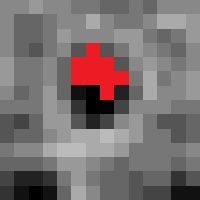
\includegraphics[height=150pt]{images/image43.jpg}
	\end{figure}
\end{frame}
\begin{frame}{Finding Holes - Example}
	\begin{figure}
		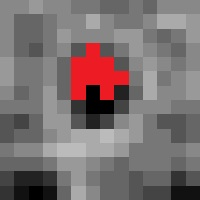
\includegraphics[height=150pt]{images/image44.jpg}
	\end{figure}
\end{frame}
\begin{frame}{Finding Holes - Example}
	\begin{figure}
		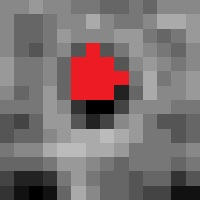
\includegraphics[height=150pt]{images/image45.jpg}
	\end{figure}
\end{frame}
\begin{frame}{Finding Holes - Example}
	\begin{figure}
		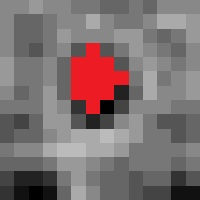
\includegraphics[height=150pt]{images/image46.jpg}
	\end{figure}
\end{frame}
\begin{frame}{Finding Holes - Example}
	\begin{figure}
		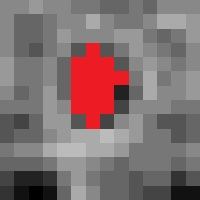
\includegraphics[height=150pt]{images/image47.jpg}
	\end{figure}
\end{frame}
\begin{frame}{Finding Holes - Example}
	\begin{figure}
		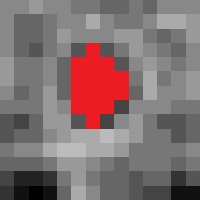
\includegraphics[height=150pt]{images/image48.jpg}
	\end{figure}
\end{frame}
\begin{frame}{Finding Holes - Example}
	\begin{figure}
		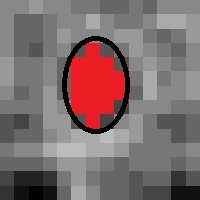
\includegraphics[height=150pt]{images/image49.jpg}
	\end{figure}
\end{frame}

\begin{frame}{Characterizing Holes}
	\begin{columns}
		\column{.6\textwidth}
		\begin{itemize}
			\item
			Once hole is found can fit a general ellipse
			\item 
			Distribution of diameter and skew of holes tells us about quality
			
			\begin{figure}
				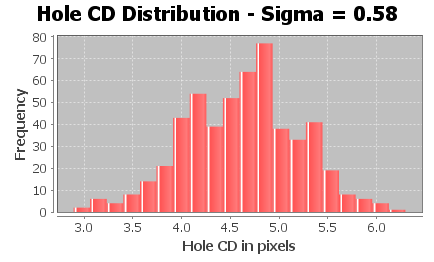
\includegraphics[height=85pt]{images/cd_dist.png}
			\end{figure}
		\end{itemize}
		\column{.4\textwidth}	
			\begin{figure}
				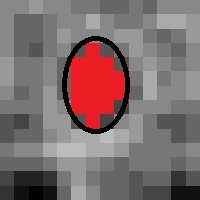
\includegraphics[height=75pt]{images/image49.jpg}
			\end{figure}
			\begin{figure}
				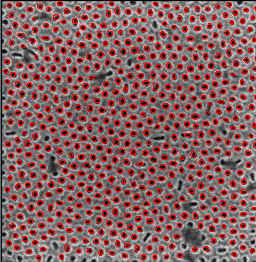
\includegraphics[height=75pt]{images/image50.png}
			\end{figure}
	\end{columns}
	
\end{frame}

\subsection{Finding Defects}
\begin{frame}{Triangulation}
	\begin{columns}
		\column{.4\textwidth}
			\begin{itemize}
				\item
				By using triangulation we can find defects in the sample
				\item
				The number of neighbours highlights missing holes
				\item
				The neighbour - neighbour distance shows irregularities / smudges
			\end{itemize}
		\column{.6\textwidth}
			\begin{figure}
				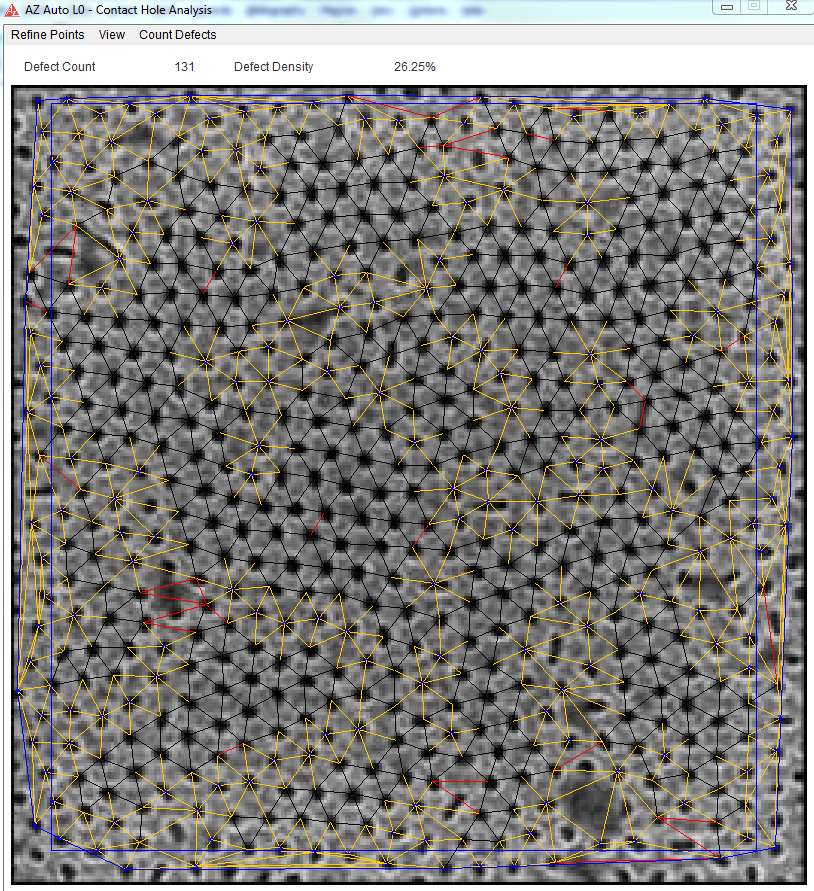
\includegraphics[height=175pt]{images/triangulation.PNG}
			\end{figure}
	\end{columns}

\end{frame}

\begin{frame}{Defect - Example}
	\begin{figure}
		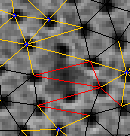
\includegraphics[height=150pt]{images/hole_defect_1.png}
		\caption{Example triangulation finding a missing hole}
	\end{figure}
\end{frame}

\section{Summary}

\begin{frame}{Summary}
	\begin{itemize}
		\item
		A system was developed in Java to reliably characterize samples of patterned silicon wafers
		\item
		Both line and hole patterns were tackled
		\item
		The R\&D team used this software to improve confidence in measurements and reduce time taken to analyse samples
	\end{itemize}
\end{frame}


\begin{frame}
	\centering
		 Questions ?
\end{frame}

\begin{frame}
	\centering
		Thank You
\end{frame}



\end{document}


